\subsection{Generador de funciones}

La onda exponencial generada en un circuito astable puede ser cambiada a un una onda triangular reemplazando el circuito RC con un integrador cómo se muestra en la ilustración . El integrador ocaciona que el capacitor se cargue y descargue de manera lineal, obteniendo de esta forma una onda triangular. \cite[pag. ~1366]{sedra-smith}

\begin{ilustracion}[ht]
    \centering
    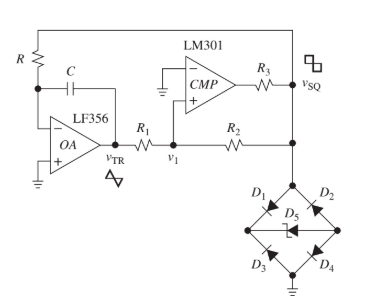
\includegraphics[width=0.5\textwidth]{marco-teorico/generador-funciones.png}
    \caption{Generador de funciones}
\end{ilustracion}

Supongamos que en la salida $V_{SQ}$ del circuito tenemos valores máximos $V_{SQ+}$ y mínimos $V_{SQ-}$, Cuando el valor de la salida es $V_{SQ+}$ una corriente es $V_{SQ+}/R$ va a pasar a traves de la resistencia y del condensador, causando que en la salida del integrador decrezca linealmente con una pendiente $-V_{SQ+}/RC$, Esto va a ocurrir hasta que la salida del integrador alcance el límite inferior del circuito astable, punto en el cual es circuito astable cambiará de estado, volviendose la salida del astable igual a $V_{SQ-}$. En este momento la corriente a traves de R y C cambiará de dirección y su valor se volverá $-V_{SQ-}/R$, causando que la salida del integrador aumente linealmente con una pendiente $V_{SQ-}/RC$ hasta que alcance el límite superior del circuito astable, punto en el cual el circuito astable cambiará de estado, volviendose la salida del astable igual a $V_{SQ+}$, una vez alcanzado este punto el circuito cambiará de estado nuevamente, haciendo que el voltaje en su salida sea $V_{SQ+}$ y repitiendo el ciclo.

De lo dicho anteriormente se puede deducir una expresión para el periodo $T$ de la onda triangular y la onda cuadrada. Durante el intervalo $T_1$ tenemos

\begin{equation*}
    \frac{V_{TH} - V_{TL}}{T_1} = \frac{V_{SQ+}}{RC}
\end{equation*}

de donde podemos despejar $T_1$

\begin{equation}
    T_1 = \frac{V_{TH} - V_{TL}}{V_{SQ+}}RC
    \label{eq:t1}
\end{equation}

De manera similar, durante $T_2$ tenemos

\begin{equation*}
    \frac{V_{TH} - V_{TL}}{T_2} = \frac{-V_{SQ-}}{RC}
\end{equation*}

de donde podemos despejar $T_2$

\begin{equation}
    T_2 = \frac{V_{TH} - V_{TL}}{-V_{SQ-}}RC
\end{equation}